\begin{figure*}[h]
\begin{center}
\begin{tabular}{p{0.2\textwidth}p{0.2\textwidth}p{0.4\textwidth}}
{\sf \large A} &
{\sf \large B} &
{\sf \large C} \\
\vspace{0pt} 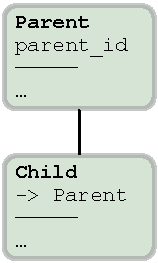
\includegraphics{./figures/depA.pdf} &
\vspace{0pt} 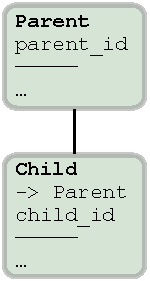
\includegraphics{./figures/depB.pdf} &
\vspace{0pt} 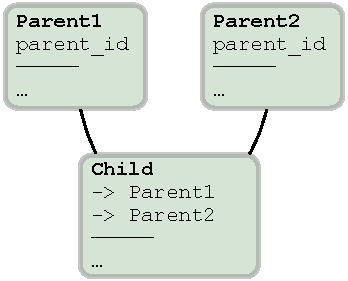
\includegraphics{./figures/depC.pdf}
\end{tabular}
\end{center}
\caption{
{\bf Three common replationships defined through the dependencies and primary keys of base relations.}
{\sf A.} A one-to-one relationship.
{\sf B.} A one-to-many (hierarchical) relationship.
{\sf C.} A combinatorial relationship. 
}
\label{dep}
\end{figure*}
